\begin{center}
	ĐỀ ÔN TẬP KIỂM TRA GIỮA HỌC KỲ I – MÔN VẬT LÝ 11\\
	Thời gian làm bài: 50 phút \\
	(Không kể thời gian phát đề)\\
\end{center}
\ANSMCQ{
	\begin{center}
		\begin{tabular}{|m{2.8em}|m{2.8em}|m{2.8em}|m{2.8em}|m{2.8em}|m{2.8em}|m{2.8em}|m{2.8em}|m{2.8em}|m{2.8em}|}
			\hline
			1D & 2D & 3B & 4A & 5D & 6C & 7C & 8A & 9D & 10A\\
			\hline
			11D & 12A & 13D & 14C & 15D & 16B & 17C & 18B & 19B & 20B\\
			\hline
			21C & 22BC & 23C & 24D & 25B & 26C & 27C & 28B & 29D & 30C\\
			\hline
		\end{tabular}
\end{center}}
\begin{enumerate}[label=\bfseries Câu \arabic*:]
	\item Đại lương cho biết số dao động mà vật thực hiện được trong $\SI{1}{\second}$ gọi là
	\begin{mcq}(4)
		\item pha dao động.
		\item tần số góc.
		\item biên độ.
		\item li độ.
	\end{mcq}
	\hideall{
		\textbf{Đáp án B.}
	}
	
	\item Trong dao động điều hòa thì nhóm đại lượng nào sau đây không thay đổi theo thời gian?
	\begin{mcq}(2)
		\item Li độ và thời gian.
		\item Biên độ và tần số góc.
		\item Li độ và pha ban đầu.
		\item Tần số và pha dao động.
	\end{mcq}
	\hideall{
		\textbf{Đáp án B.}
	}
	
	\item Một chất điểm dao động điều hoà với phương trình $x=\xsi{10\cos\left(15t+\pi\right)}{\centi\meter}$ ($x$ tính bằng $\si{\centi\meter}$, $t$ tính bằng giây). Chất điểm này dao động với tần số góc là
	\begin{mcq}(4)
		\item $\SI{20}{\radian/\second}$.
		\item $\SI{10}{\radian/\second}$.
		\item $\SI{5}{\radian/\second}$.
		\item $\SI{15}{\radian/\second}$.
	\end{mcq}
	\hideall{
		\textbf{Đáp án D.}
	}
	
	\item Một chất điểm chuyển động tròn đều trên một đường tròn bán kính $R$, tốc độ góc $\omega
	$. Hình chiếu của chất điểm này lên đường kính là một dao động điều hoà có
	\begin{mcq}(2)
		\item biên độ $R$.
		\item biên độ $2R$.
		\item pha ban đầu $\omega t$.
		\item chiều dài quỹ đạo $4R$.
	\end{mcq}
	\hideall{
		\textbf{Đáp án D.}
	}
	
	\item Một chất điểm dao động điều hoà với phương trình $x=\xsi{5\cos\left(10\pi t+\dfrac{\pi}{3}\right)}{\centi\meter}$. Li độ của vật khi pha dao động bằng $\xsi{\pi}{\radian}$ là
	\begin{mcq}(4)
		\item $\SI{5}{\centi\meter}$.
		\item $\SI{-5}{\centi\meter}$.
		\item $\SI{2.5}{\centi\meter}$.
		\item $\SI{-2.4}{\centi\meter}.$
	\end{mcq}
	\hideall{
		\textbf{Đáp án B.}\\
		Khi pha dao động là $\varphi=\xsi{\pi}{\radian}$ thì li độ dao động của vật là
		$$x=5\cos\pi=-\SI{5}{\centi\meter}.$$
	}
	
	\item Một chất điểm dao động điều hòa trong 10 dao động toàn phần đi được quãng đường $\SI{120}{\centi\meter}$. Quỹ đạo của dao động có chiều dài là
	\begin{mcq}(4)
		\item $\SI{6}{\centi\meter}$.
		\item $\SI{12}{\centi\meter}$.
		\item $\SI{3}{\centi\meter}$.
		\item $\SI{9}{\centi\meter}$.
	\end{mcq}
	\hideall{
		\textbf{Đáp án C.}\\
		Biên độ dao động của chất điểm:
		$$A=\dfrac{s}{4\cdot10}=\SI{3}{\centi\meter}$$
		Chiều dài quỹ đạo:
		$$L=2A=\SI{6}{\centi\meter}.$$
	}
	
	\item Trong một trò chơi bắn súng, một khẩu súng bắn vào mục tiêu di động. Súng tự nhả đạn theo thời gian một cách ngẫu nhiên. Người chơi phải chĩa súng theo một hướng nhất định còn mục tiêu dao động điều hoà theo phương ngang như hình vẽ. Người chơi cần chĩa súng vào vùng nào để có thể ghi được số lần trúng nhiều nhất?
	\begin{center}
		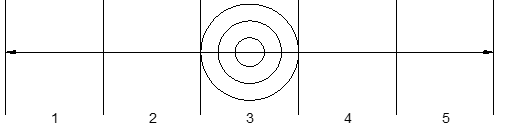
\includegraphics[width=0.5\linewidth]{../figs/D11-4-1}
	\end{center}
	\begin{mcq}(2)
		\item vùng 3.
		\item vùng 1 hoặc vùng 5.
		\item vùng 2 hoặc 4.
		\item bất kì vùng nào.
	\end{mcq}
	\hideall{
		\textbf{Đáp án B.}\\
		Tốc độ của vật ở vị trí biên là nhỏ nhất, thời gian vật ở vùng 1 và vùng 5 cũng lớn hơn so với các vùng khác nên xác suất ghi điểm ở vùng 1 và 5 là cao nhất.
	}
	
	\item Một vật dao động điều hoà phải mất $\SI{0.025}{\second}$ để đi từ điểm có vận tốc bằng không đến điểm tiếp theo cũng có vận tốc bằng không, hai điểm ấy cách nhau $\SI{10}{\centi\meter}$. Chọn phát biểu đúng.
	\begin{mcq}(4)
		\item Chu kì dao động là $\SI{0.025}{\second}$.
		\item Tần số dao động là $\SI{10}{\hertz}$.
		\item Biên độ dao động là $\SI{10}{\centi\meter}$.
		\item Vận tốc của vật có độ lớn cực đại là $\xsi{2\pi}{\meter/\second}$.
	\end{mcq}
	\hideall{
		\textbf{Đáp án D.}\\
		Vật có vận tốc bằng 0 khi ở vị trí biên. Như vậy ta có
		$$\dfrac{T}{2}=\SI{0.025}{\second}\Rightarrow T=\SI{0.05}{\second};\quad A=\SI{5}{\centi\meter}$$
		Vận tốc cực đại của vật:
		$$v_\text{max}=\omega A=\dfrac{2\pi}{T}\cdot A=\dfrac{2\pi}{\SI{0.05}{\second}}\cdot\left(\SI{0.05}{\meter}\right)=\xsi{2\pi}{\meter/\second}.$$
	}
	
	\item Một vật dao động điều hoà với phương trình li độ $x=A\cos\left(\omega t+\varphi_0\right)$. Gọi $v$ là vận tốc của vật khi vật ở vị trí li độ $x$. Biên độ dao động của vật là
	\begin{mcq}(4)
		\item $\sqrt{x^2+\dfrac{v^4}{\omega^2}}$.
		\item $\sqrt{x^2+\dfrac{v^2}{\omega^2}}$>
		\item $\sqrt{x^2+\dfrac{v^2}{\omega^4}}$.
		\item $\sqrt{x+\dfrac{v^2}{\omega^2}}$.
	\end{mcq}
	\hideall{
		\textbf{Đáp án B.}
	}
	
	\item Một chất điểm dao động điều hoà với tần số bằng $\SI{4}{\hertz}$ và biên độ bằng $\SI{10}{\centi\meter}$. Gia tốc cực đại của chất điểm bằng
	\begin{mcq}(4)
		\item $\SI{25}{\centi\meter/\second^2}$.
		\item $\SI{2.5}{\meter/\second^2}$.
		\item $\SI{63.2}{\meter/\second}$.
		\item $\SI{6.32}{\meter/\second^2}$.
	\end{mcq}
	\hideall{
		\textbf{Đáp án C.}\\
		Gia tốc cực đại của vật là
		$$a_\text{max}=\omega^2 A=\left(2\pi f\right)^2A\approx\SI{63.2}{\meter/\second^2}.$$
	}
	
	\item Một chất điểm dao động điều hoà có phương trình vận tốc $v=\xsi{20\pi \cos\left(2\pi t+\dfrac{\pi}{6}\right)}{\centi\meter/\second}$. Phương trình dao động của chất điểm có dạng 
	\begin{mcq}(2)
		\item $x=\xsi{10\cos\left(2\pi t-\dfrac{\pi}{3}\right)}{\centi\meter}.$
		\item $x=\xsi{10\cos\left(2\pi t+\dfrac{2\pi}{3}\right)}{\centi\meter}.$
		\item $x=\xsi{20\cos\left(2\pi t+\dfrac{5\pi}{6}\right)}{\centi\meter}.$
		\item $x=\xsi{20\cos\left(2\pi t+\dfrac{\pi}{3}\right)}{\centi\meter}.$
	\end{mcq}
	\hideall{
		\textbf{Đáp án A.}\\
		Biên độ dao động của chất điểm:
		$$A=\dfrac{v_\text{max}}{\omega}=\SI{10}{\centi\meter}.$$
		Pha ban đầu của dao động:
		$$\varphi_{0x}=\varphi_{0v}-\dfrac{\pi}{2}=-\xsi{\dfrac{\pi}{3}}{\radian}$$
		Phương trình li độ của chất điểm:
		$$x=\xsi{10\cos\left(2\pi t-\dfrac{\pi}{3}\right)}{\centi\meter}.$$
	}
	
	\item Một chất điểm dao động điều hoà trên trục $Ox$. Tại thời điểm $t_1$, $t_2$ vật có vận tốc và gia tốc lần lượt là $v_1=\xsi{10\sqrt{3}}{\centi\meter/\second}$; $a_1=\SI{-1}{\meter/\second^2}$; $v_2=\SI{-10}{\centi\meter/\second}$; $a_2=\xsi{\sqrt{3}}{\meter/\second^2}$. Tốc độ cực đại của vật bằng
	\begin{mcq}(4)
		\item $\SI{20}{\centi\meter/\second}$.
		\item $\SI{40}{\centi\meter/\second}$.
		\item $\xsi{10\sqrt{5}}{\centi\meter/\second}$.
		\item $\xsi{20\sqrt{3}}{\centi\meter/\second}.$
	\end{mcq}
	\hideall{
		\textbf{Đáp án A.}\\
		Áp dụng hệ thức độc lập thời gian
		$$\dfrac{v^2}{v^2_\text{max}}+\dfrac{a^2}{a^2_\text{max}}=1\Rightarrow\dfrac{1}{a^2_\text{max}}=\dfrac{1-\dfrac{v^2}{v^2_\text{max}}}{a^2}$$
		Như vậy:
		$$\dfrac{1-\dfrac{v^2_1}{v^2_\text{max}}}{a^2_1}=\dfrac{1-\dfrac{v^2_2}{v^2_\text{max}}}{a^2_2}\Rightarrow v_\text{max}=\SI{20}{\centi\meter/\second}.$$
	}
\end{enumerate}